\documentclass[12pt,tikz,border=8pt]{standalone}
\usepackage{libertine}
\usepackage{amsmath,amssymb}
\usepackage{tikz}
\usetikzlibrary{arrows.meta}

\begin{document}
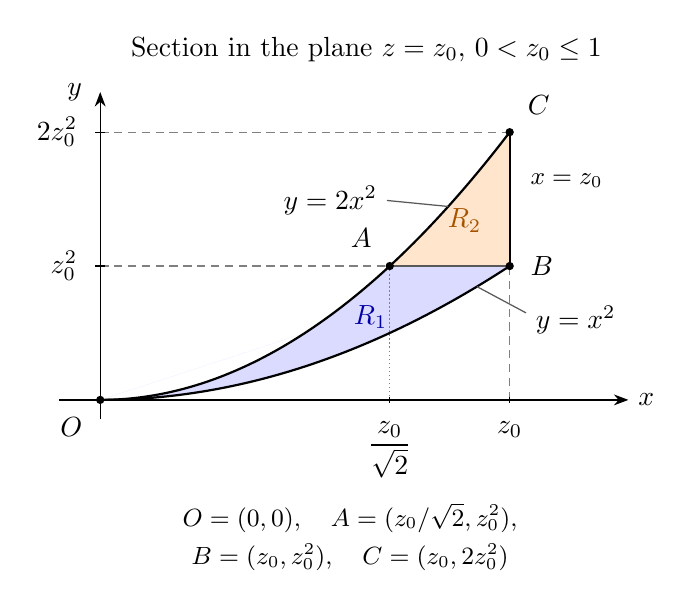
\begin{tikzpicture}[x=5.2cm,y=1.7cm,>=Stealth,
  boundary/.style={black,line width=0.8pt},
  guide/.style={gray,densely dashed,line width=0.45pt},
  every node/.style={font=\normalsize}]
  % Normalized drawing coordinates X=x/z_0 and Y=y/z_0^2.
  % The actual axis labels and all marked coordinates remain symbolic.
  \def\a{0.7071067812}

  % R_1: the part of x^2 <= y <= 2x^2 with y <= z_0^2.
  \fill[blue!14]
    (0,0) plot[domain=0:\a,samples=65] (\x,{2*\x*\x})
    -- (1,1)
    plot[domain=1:0,samples=80] (\x,{\x*\x}) -- cycle;
  % R_2: the remaining part, above y=z_0^2 and left of x=z_0.
  \fill[orange!20]
    (\a,1) plot[domain=\a:1,samples=55] (\x,{2*\x*\x})
    -- (1,1) -- cycle;

  \draw[->,line width=0.5pt] (-0.10,0) -- (1.29,0)
    node[right] {$x$};
  \draw[->,line width=0.5pt] (0,-0.14) -- (0,2.30)
    node[left=3pt] {$y$};
  \draw[guide] (0,1) -- (\a,1);
  \draw[guide] (0,2) -- (1,2);
  \draw[guide] (1,0) -- (1,1);
  \draw[gray,densely dotted,line width=0.45pt] (\a,0) -- (\a,1);

  \draw[boundary,domain=0:1,samples=100]
    plot (\x,{\x*\x});
  \draw[boundary,domain=0:1,samples=100]
    plot (\x,{2*\x*\x});
  \draw[boundary] (1,1) -- (1,2);
  \draw[black!65,line width=0.65pt] (\a,1) -- (1,1);

  \draw (\a,0.025) -- (\a,-0.025)
    node[below=3pt] {$\dfrac{z_0}{\sqrt2}$};
  \draw (1,0.025) -- (1,-0.025) node[below=3pt] {$z_0$};
  \draw (0.012,1) -- (-0.012,1) node[left=3pt] {$z_0^2$};
  \draw (0.012,2) -- (-0.012,2) node[left=3pt] {$2z_0^2$};

  \fill (0,0) circle[radius=1.5pt] node[below left=3pt] {$O$};
  \fill (\a,1) circle[radius=1.5pt] node[above left=3pt] {$A$};
  \fill (1,1) circle[radius=1.5pt] node[right=4pt] {$B$};
  \fill (1,2) circle[radius=1.5pt] node[above right=3pt] {$C$};

  \node[blue!65!black] at (0.66,0.62) {$R_1$};
  \node[orange!65!black] at (0.89,1.34) {$R_2$};
  \node[right=4pt,font=\small] at (1,1.64) {$x=z_0$};
  \node[left] at (0.70,1.49) {$y=2x^2$};
  \draw[black!65,line width=0.45pt] (0.70,1.49) -- (0.85,1.445);
  \node[right] at (1.04,0.60) {$y=x^2$};
  \draw[black!65,line width=0.45pt] (1.04,0.65) -- (0.92,0.8464);

  \node at (0.65,2.62) {Section in the plane $z=z_0$, $0<z_0\leq1$};
  \node[align=center,anchor=north,font=\small] at (0.61,-0.70) {
    $O=(0,0),\quad A=(z_0/\sqrt2,z_0^2),$\\[3pt]
    $B=(z_0,z_0^2),\quad C=(z_0,2z_0^2)$
  };
\end{tikzpicture}
\end{document}
